\documentclass[11pt, a4paper]{article}

\usepackage[margin=1in]{geometry}
\usepackage[utf8]{inputenc}
\usepackage[T1]{fontenc}
\usepackage[english]{babel}
\usepackage{amsmath}
\usepackage{amssymb}
\usepackage{graphicx}
\usepackage{booktabs}
\usepackage{microtype}
\usepackage{hyperref}
\usepackage{caption}
\usepackage{enumitem}
\usepackage{longtable}

\captionsetup{font=small, labelfont=bf, skip=6pt}
\setlist[itemize]{leftmargin=1.5em, itemsep=0.3em, topsep=0.4em}
\setlength{\LTpre}{0.75em}
\setlength{\LTpost}{0.75em}
\renewcommand{\arraystretch}{1.1}
\hypersetup{
    colorlinks=true,
    linkcolor=black,
    citecolor=black,
    urlcolor=blue
}

\title{The Impact of Short-term Intensity and Tactical Behavior on Goal-Scoring Probability: A Machine Learning Approach}
\author{
    Jakub Piotrowski \and Jakub Szulc \and Mateusz Jastrzebski \\
    \vspace{0.2cm}
    \textit{Polish-Japanese Academy of Information Technology}
}
\date{\today}

\begin{document}
\maketitle

\begin{abstract}
We study rare-event prediction of whether a player scores after a 15-minute match checkpoint. The dataset contains 3,486 checkpoint rows (203 positives, 5.82\%) across 31 fixtures and is enriched with event logs (passes, runs, shots, pressure actions). We use fold-safe temporal feature engineering, grouped cross-validation by fixture, and a stacking ensemble over out-of-fold probabilities from logistic regression, Extra Trees, Random Forest, XGBoost, and LightGBM. In the refreshed run (\texttt{fast} preset, 3 grouped folds, no XGBoost HPO, AutoGluon holdout enabled), the strongest single OOF PR-AUC is Random Forest (0.120), while stacking attains the highest ROC-AUC (0.682) and best OOF Brier score (0.054). Results confirm that short-term and cumulative in-match behaviors carry measurable signal, but absolute minority-class separability remains limited, consistent with football's low-scoring stochastic nature.
\end{abstract}

\section{Introduction}
Modern football analytics can explain action value well, but forecasting an individual player's scoring event from in-match state alone remains difficult. This work focuses on \emph{checkpoint-time} prediction: for each player appearance at regular checkpoints, estimate the probability of scoring later in the match using only information available up to that checkpoint.

The primary contribution is a fully leakage-aware pipeline: temporal filtering by absolute match time, grouped validation by fixture, fold-local feature fitting/encoding, and explicit exclusion of future-known substitution fields from the model feature set.

\section{Data and Problem Setup}

\subsection{Raw data}
\begin{longtable}{lrrlp{0.34\linewidth}}
\caption{Dataset overview (raw CSVs).}
\label{tab:dataset_overview} \\
\toprule
Dataset & Rows & Columns & Unique player appearances & Role \\
\midrule
Checkpoints & 3,486 & 33 & 869 & Main modeling table \\
Passes & 29,795 & 7 & 959 & Passing context \\
Runs & 35,133 & 10 & 968 & Physical context \\
Shots & 780 & 12 & 453 & Shooting context \\
Pressure & 12,185 & 10 & 923 & Pressed-action context \\
\bottomrule
\end{longtable}

Target variable: \texttt{scored\_after}. In the training-ready checkpoint table: 203 positives and 3,283 negatives (5.82\% positive rate).

\subsection{Exploratory distributions}
\begin{figure}[htbp]
\centering
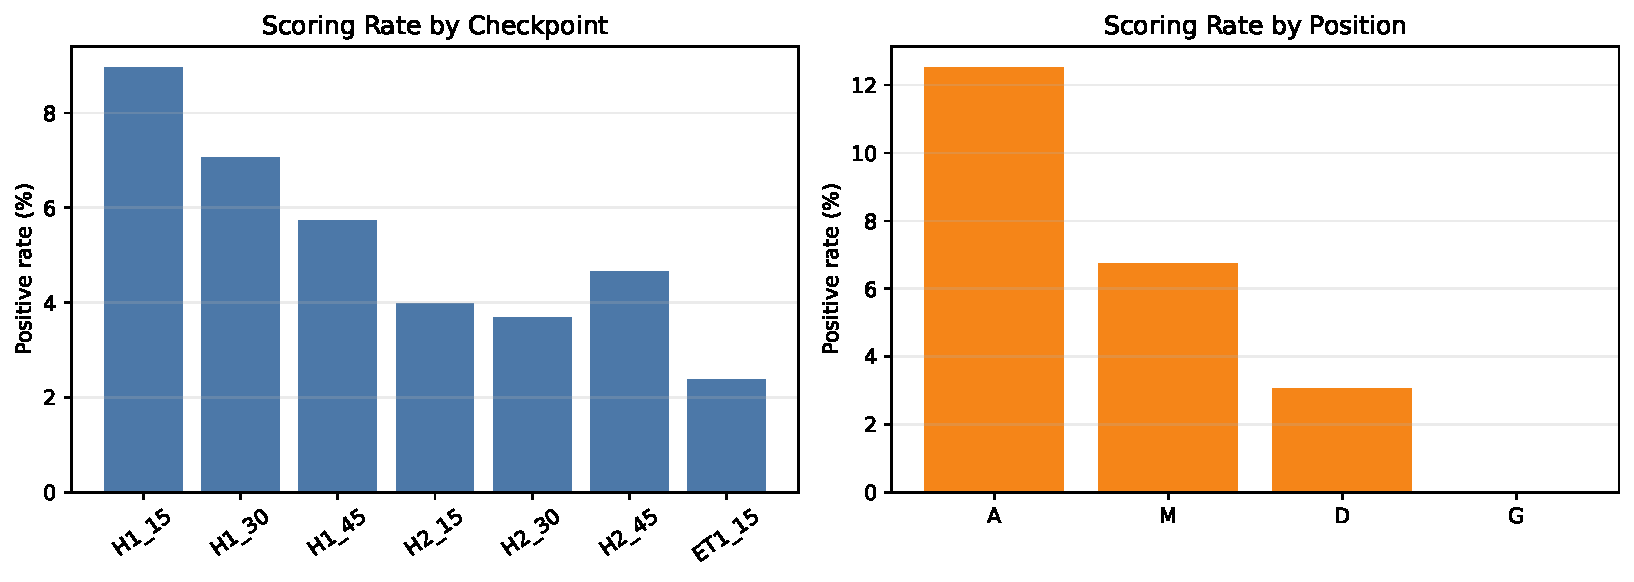
\includegraphics[width=0.92\linewidth]{figures/target_rates.pdf}
\caption{Scoring rate by checkpoint and position.}
\label{fig:target_rates}
\end{figure}

\begin{figure}[htbp]
\centering
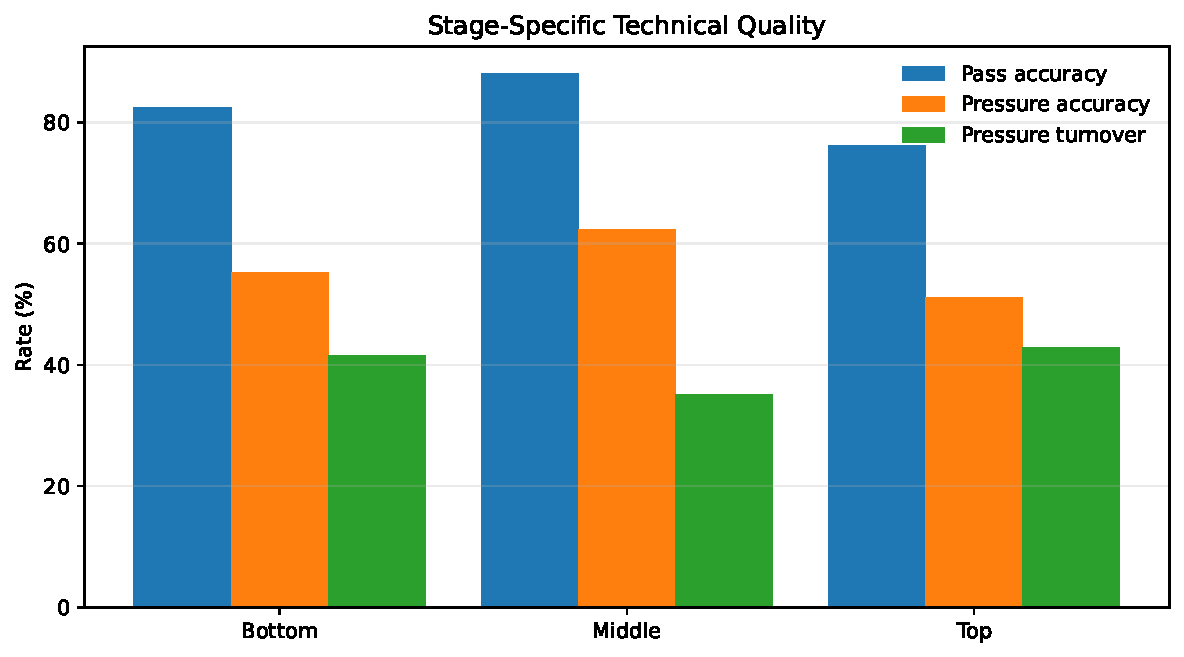
\includegraphics[width=0.92\linewidth]{figures/event_stage_quality.pdf}
\caption{Pass accuracy and pressure outcomes by pitch stage.}
\label{fig:event_stage_quality}
\end{figure}

\section{Preprocessing and Leakage Controls}

\subsection{Training-row validation}
Before feature modeling, checkpoint rows are validated with temporal leakage checks and on-pitch filtering:
\begin{itemize}
    \item temporal boundaries are validated against event logs;
    \item rows where \texttt{is\_on\_pitch} is false are dropped;
    \item training aborts if no valid rows remain.
\end{itemize}

\subsection{Fold-safe temporal features}
Features are built inside each CV fold via \texttt{TemporalFeatureBuilder}:
\begin{itemize}
    \item per-fold fit on training checkpoints only;
    \item transform applied separately to train/validation partitions;
    \item event filtering uses absolute match minute:
    \[
    \texttt{minute\_in} \leq \texttt{event\_abs\_minute} \leq \texttt{checkpoint\_abs\_minute}
    \]
    with period offsets to avoid half-overlap artifacts.
\end{itemize}

\subsection{Model matrix construction}
For each fold and feature subset:
\begin{itemize}
    \item categorical columns: missing $\rightarrow$ \texttt{"missing"}, rare-level pooling (min count/share), one-hot encoding with train-to-val column alignment;
    \item additional category statistics: frequency encoding for all categoricals, plus smoothed target-rate encoding (smoothing=20) for selected columns (\texttt{position}, \texttt{formation});
    \item numeric columns: coercion to numeric and median imputation fit on train only.
\end{itemize}

\subsection{Excluded fields and feature groups}
The modeling column selector excludes identifiers, target, and known future-leaking substitution fields (\texttt{minute\_out}, \texttt{subbed}), plus \texttt{jersey\_number}. The run used 241 columns in the \texttt{all\_features} group after deterministic redundancy filtering.

\section{Modeling Setup}

\subsection{Validation protocol}
We use \texttt{StratifiedGroupKFold} grouped by \texttt{fixture\_id}. In this run: 3 folds (\texttt{fast} preset).

\subsection{Base models and stacking}
Main all-feature OOF benchmark includes:
\begin{itemize}
    \item Logistic Regression (balanced),
    \item Extra Trees,
    \item Random Forest,
    \item XGBoost,
    \item LightGBM.
\end{itemize}
Stacking trains a meta-level balanced logistic model on base-model OOF probabilities (with calibration fallback path). Fold thresholds for class predictions are selected by F1 on training fold data.

\subsection{AutoGluon benchmark}
An additional \texttt{autogluon\_holdout} row is produced from a single train/validation split, not from full OOF across all 3,486 rows. It is useful as a complementary reference but not directly comparable with full OOF lines.

\section{Results}

\subsection{OOF model performance}
\begin{table}[htbp]
\centering
\caption{All-features model comparison (OOF for main models, holdout for AutoGluon).}
\label{tab:oof_results}
\begin{tabular}{lcccc}
\toprule
Model & n & ROC-AUC & PR-AUC & Brier \\
\midrule
stacked & 3486 & 0.682 & 0.114 & \textbf{0.054} \\
random\_forest & 3486 & 0.679 & \textbf{0.120} & 0.058 \\
extra\_trees & 3486 & 0.674 & 0.114 & 0.061 \\
lightgbm & 3486 & 0.656 & 0.114 & 0.059 \\
xgboost & 3486 & 0.650 & 0.107 & 0.060 \\
logistic & 3486 & 0.580 & 0.078 & 0.186 \\
\midrule
autogluon\_holdout & 1096 & 0.661 & 0.080 & 0.047 \\
\bottomrule
\end{tabular}
\end{table}

\begin{figure}[htbp]
\centering
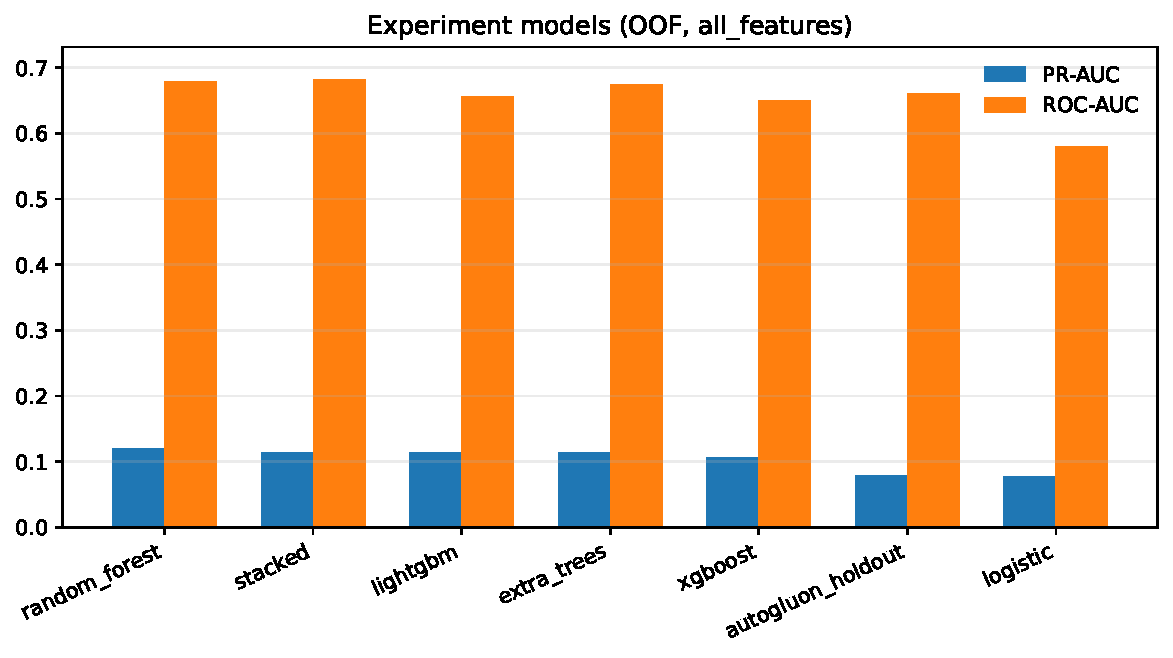
\includegraphics[width=0.92\linewidth]{figures/model_comparison.pdf}
\caption{Model ranking plot generated from experiment exports.}
\label{fig:model_comparison}
\end{figure}

\subsection{Ablation view (XGBoost feature families)}
\begin{longtable}{lccc}
\caption{XGBoost ablations from \texttt{metrics.csv}.}
\label{tab:ablations} \\
\toprule
Feature set & ROC-AUC & PR-AUC & Brier \\
\midrule
base\_checkpoint & 0.647 & 0.114 & 0.060 \\
base\_plus\_passing & 0.648 & 0.111 & 0.060 \\
base\_plus\_pressure & 0.642 & 0.108 & 0.060 \\
cumulative\_only & 0.631 & 0.108 & 0.063 \\
all\_features & 0.650 & 0.107 & 0.060 \\
recent\_only & 0.630 & 0.094 & 0.062 \\
sprints\_shots & 0.615 & 0.090 & 0.072 \\
external\_context & 0.556 & 0.071 & 0.134 \\
\bottomrule
\end{longtable}

\subsection{Feature-level interpretation}
\begin{figure}[htbp]
\centering
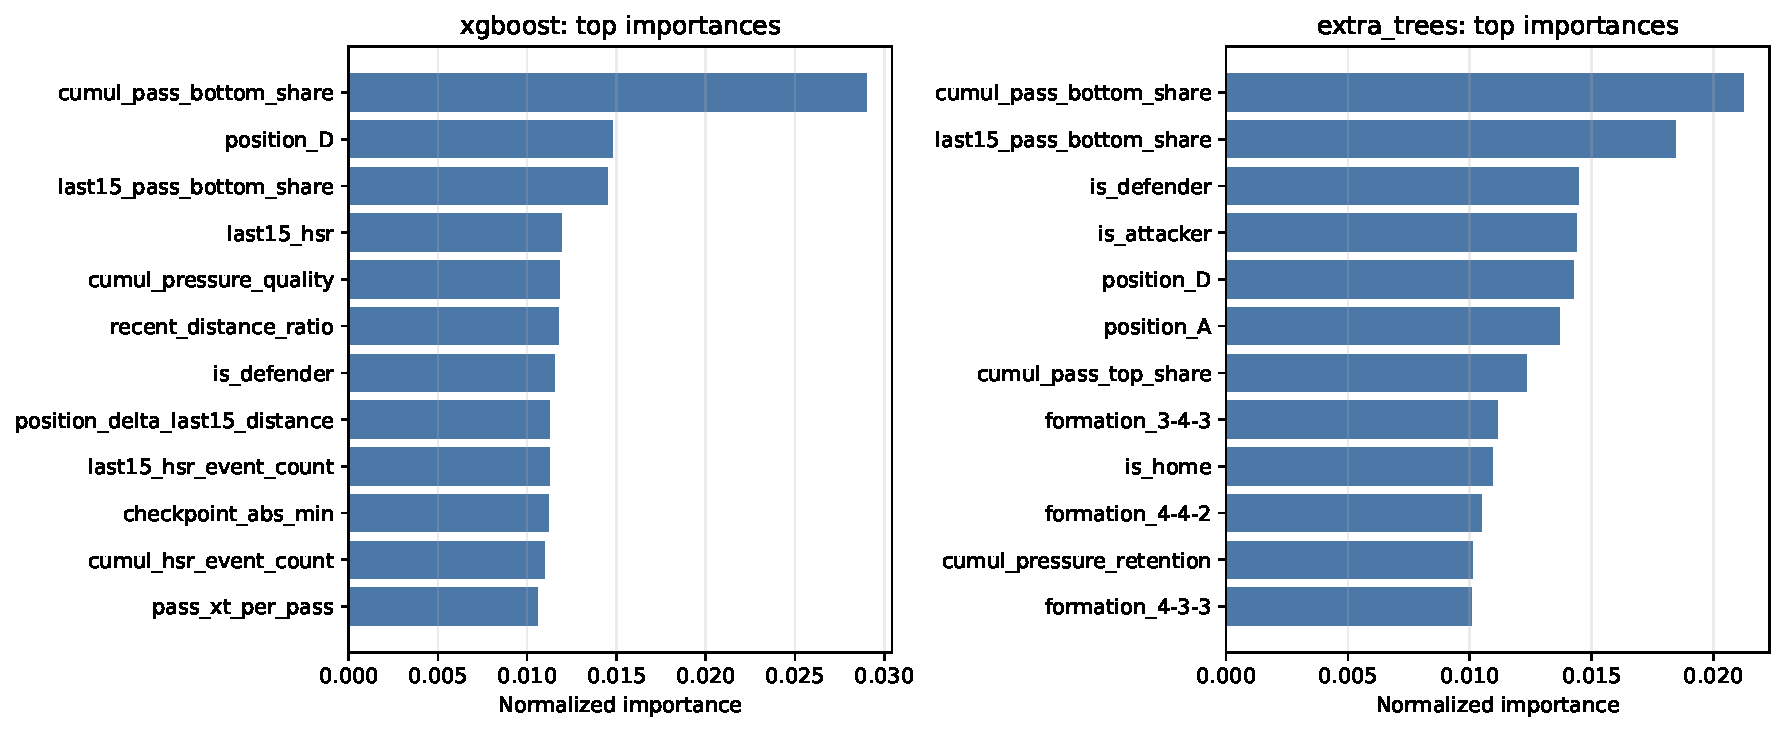
\includegraphics[width=0.92\linewidth]{figures/model_feature_importance.pdf}
\caption{Normalized feature importance plot (from report figure export).}
\label{fig:model_feature_importance}
\end{figure}

\begin{figure}[htbp]
\centering
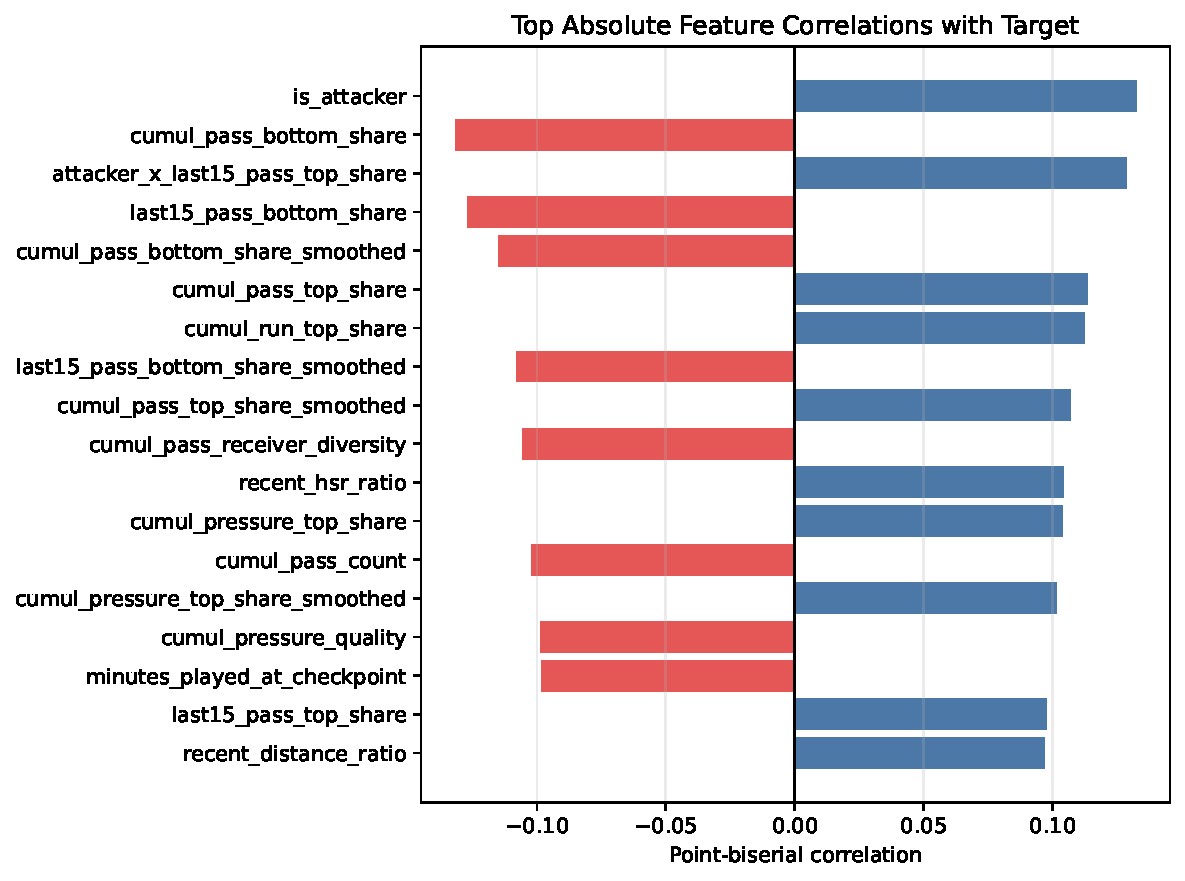
\includegraphics[width=0.92\linewidth]{figures/feature_correlations.pdf}
\caption{Top absolute correlations with \texttt{scored\_after}.}
\label{fig:feature_correlations}
\end{figure}

Most stable patterns across correlation and model-importance exports point to:
\begin{itemize}
    \item positional/territorial effects (\texttt{is\_attacker}, pass-stage shares),
    \item recent intensity signals (\texttt{recent\_hsr\_ratio}, distance ratio),
    \item pressure-context features (top-share / quality aggregates).
\end{itemize}

\subsection{Ensemble diagnostics}
\begin{figure}[htbp]
\centering
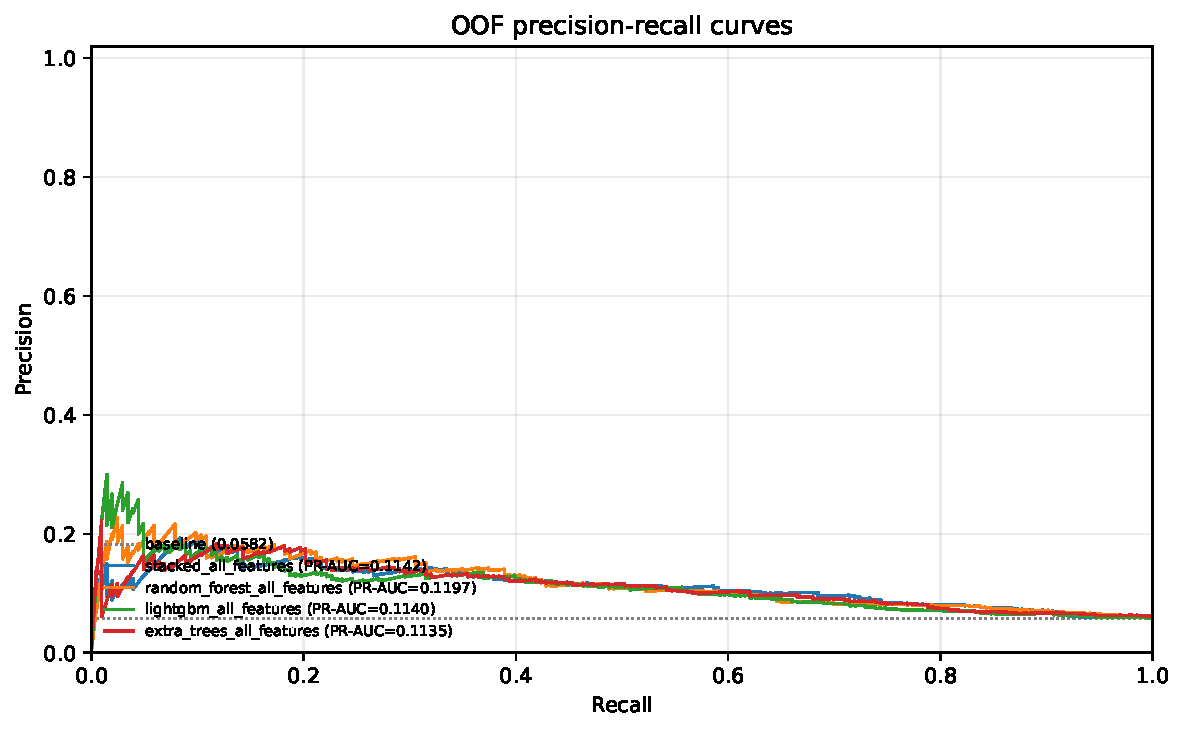
\includegraphics[width=0.92\linewidth]{figures/oof_precision_recall.pdf}
\caption{Precision-recall curves for top OOF prediction columns.}
\label{fig:oof_pr}
\end{figure}

\begin{figure}[htbp]
\centering
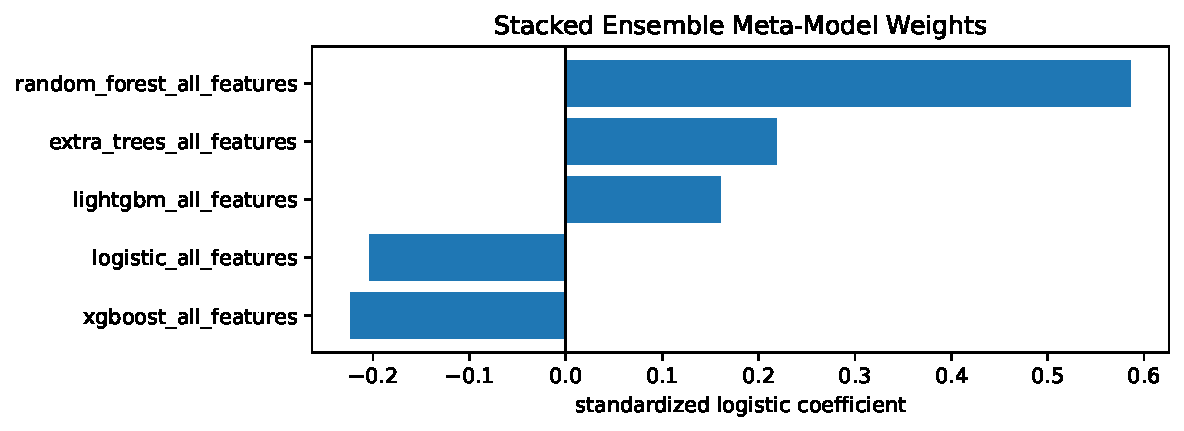
\includegraphics[width=0.82\linewidth]{figures/stacked_meta_weights.pdf}
\caption{Post-hoc standardized weights of base-model OOF columns in a diagnostic meta-logit fit.}
\label{fig:stacked_weights}
\end{figure}

\begin{table}[htbp]
\centering
\caption{Diagnostic meta-model standardized coefficients (from explainability scan).}
\label{tab:stack_weights}
\begin{tabular}{lr}
\toprule
Base prediction & Standardized weight \\
\midrule
random\_forest\_all\_features & 0.585 \\
xgboost\_all\_features & -0.223 \\
extra\_trees\_all\_features & 0.219 \\
logistic\_all\_features & -0.204 \\
lightgbm\_all\_features & 0.160 \\
\bottomrule
\end{tabular}
\end{table}

\paragraph{Important scope note.}
The explainability run used \texttt{scan} mode (fast), so expensive SHAP/permutation artifacts are placeholders in this package; practical interpretation here is based on OOF metrics, correlation exports, model importance CSV, PR curves, and stacking-weight diagnostics.

\section{Discussion}
The pipeline consistently extracts signal above base rate, but absolute PR-AUC remains low, reflecting rare-event difficulty and noisy football outcomes. In this run, Random Forest gives the strongest minority ranking (PR-AUC), while stacking improves ROC-AUC and Brier calibration relative to individual tree models. The model family differences and meta-weights indicate complementary behavior between base learners rather than one universally dominant predictor.

\section{Conclusion}
Short-term and cumulative in-match behaviors provide valid predictive signal for post-checkpoint scoring probability, but are insufficient for high-certainty forecasting in isolation. The strongest practical path forward is hybridization with macro context (player history, team/opponent strength, richer game-state variables) while preserving strict grouped temporal validation.

\end{document}
